\section{Genetic Regulatory Network Model}

\begin{frame}{Model Framework}
\begin{columns}
\begin{column}{0.5\textwidth}
\begin{figure}
    \centering
    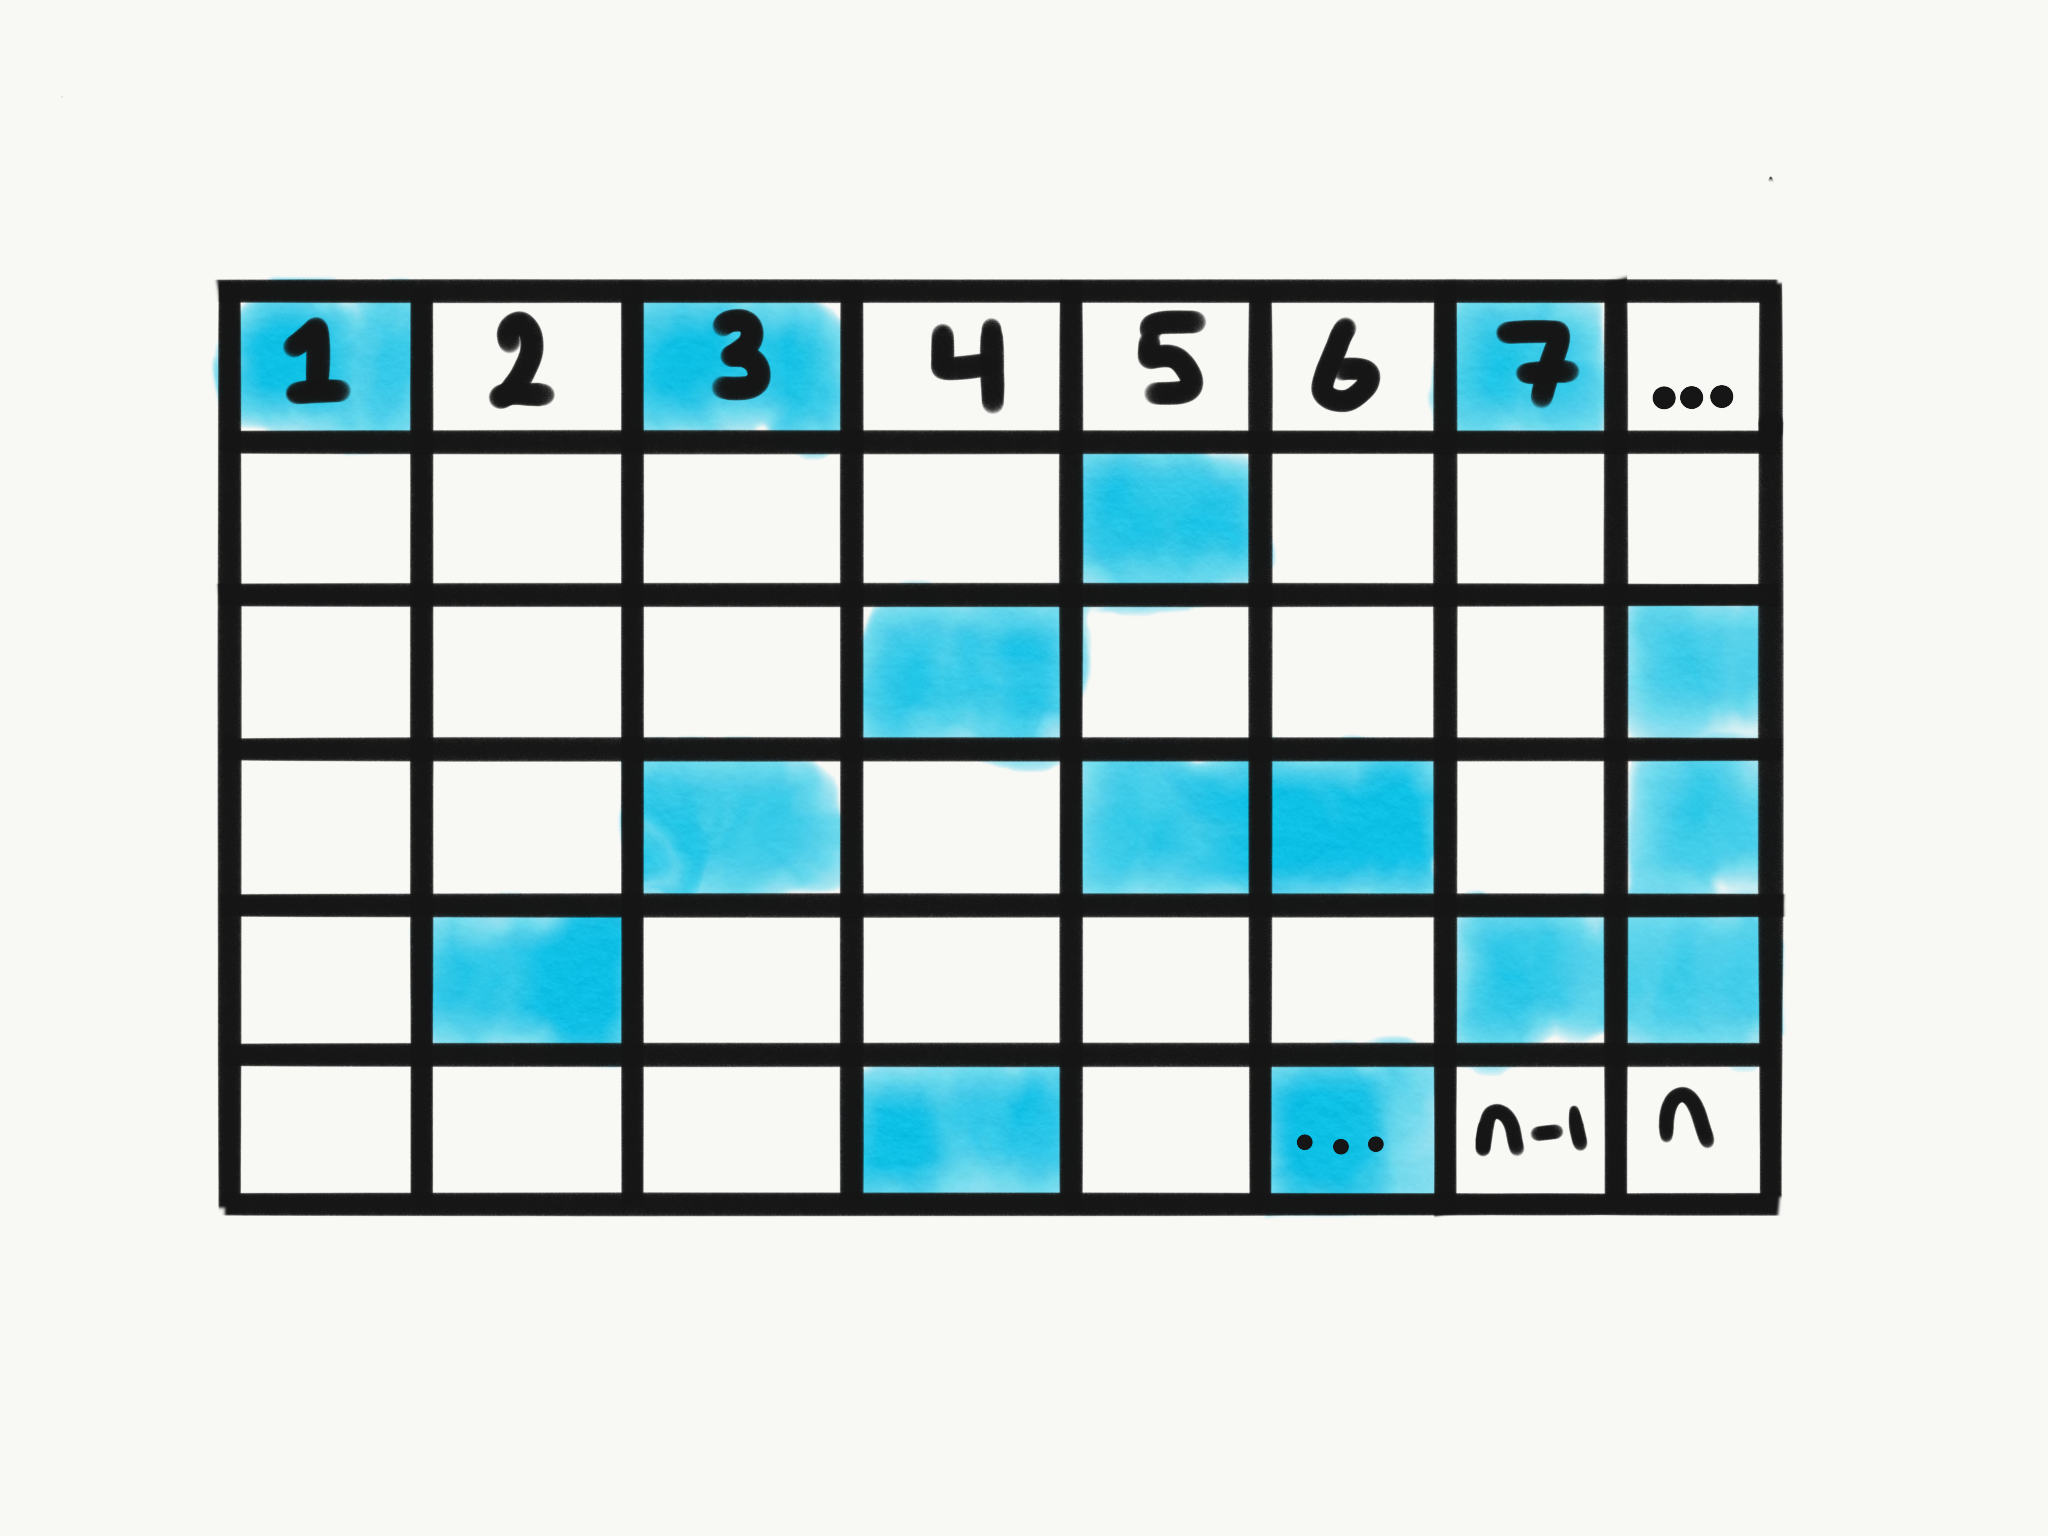
\includegraphics[width=\textwidth]{img/initial_state}
 	\captionsetup{singlelinecheck=off,justification=raggedright}
  	\caption{Chemical concentrations are represented as a list of boolean values.}
    \label{fig:initial_state}
\end{figure}
\end{column}

\begin{column}{0.5\textwidth}
\begin{figure}
    \centering
    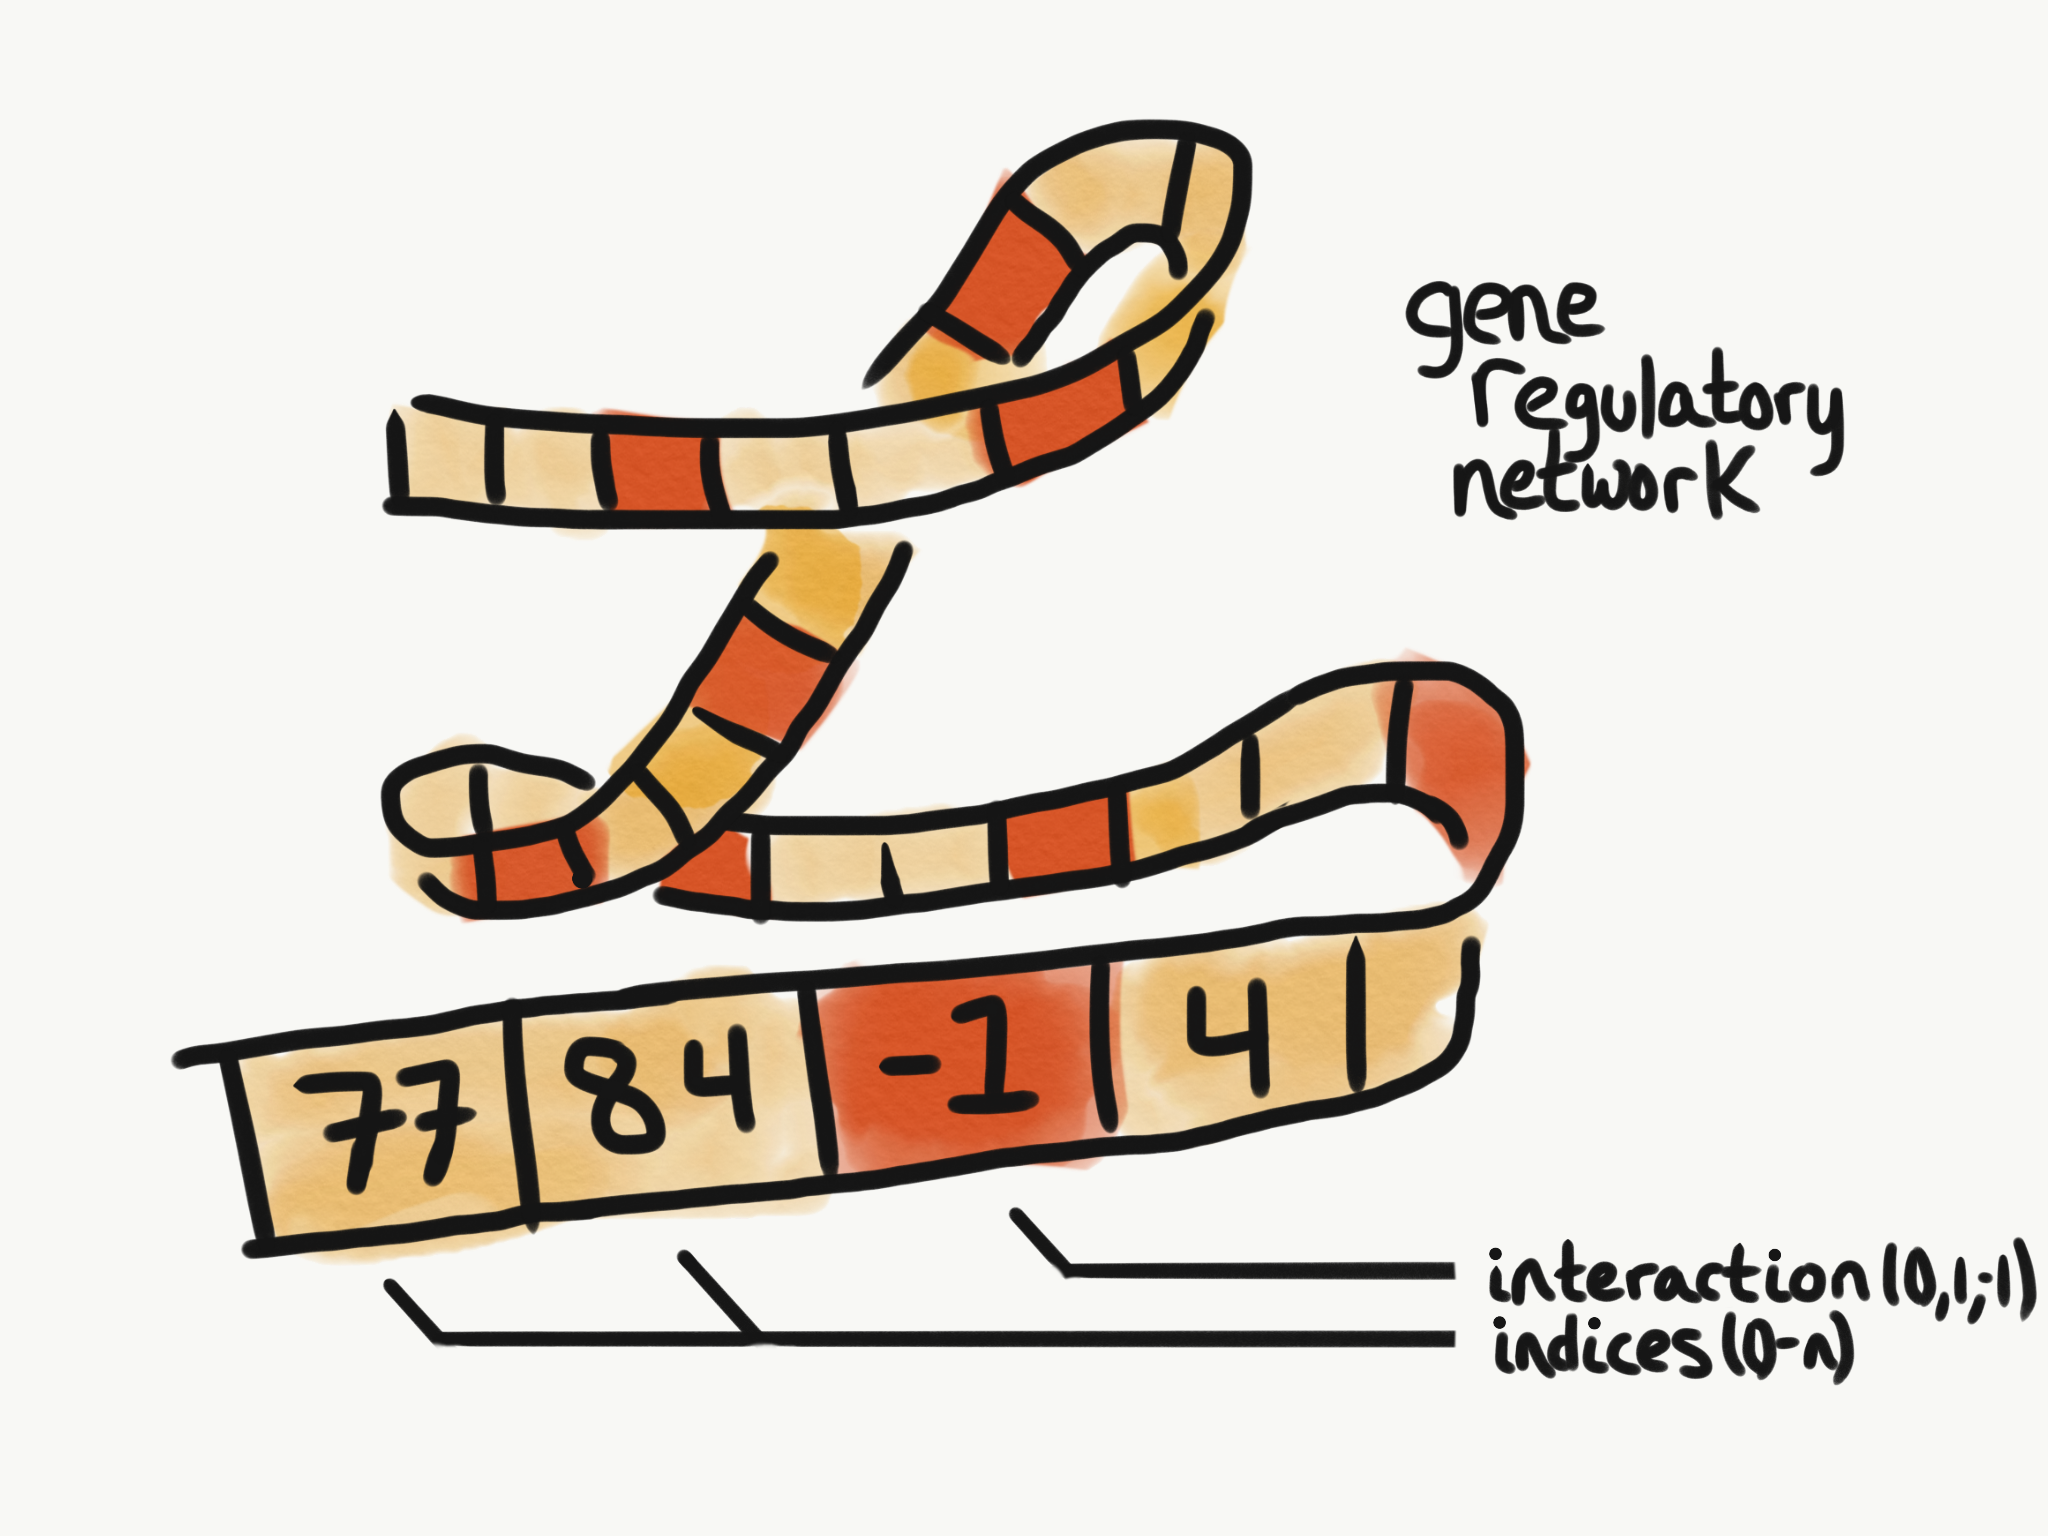
\includegraphics[width=\textwidth]{img/expanded_grn}
 	\captionsetup{singlelinecheck=off,justification=raggedright}
  	\caption{The GRN genotype is a set of if-then rules that acts on a set of chemical concentrations. The model employed was inspired by \cite{Wilder2015ReconcilingEvolvability}.}
    \label{fig:grn_list}
\end{figure}
\end{column}

\end{columns}
\end{frame}

\begin{frame}{Model Framework}
\begin{figure}
  \centering
  \begin{subfigure}[b]{\textwidth}
    \centering
    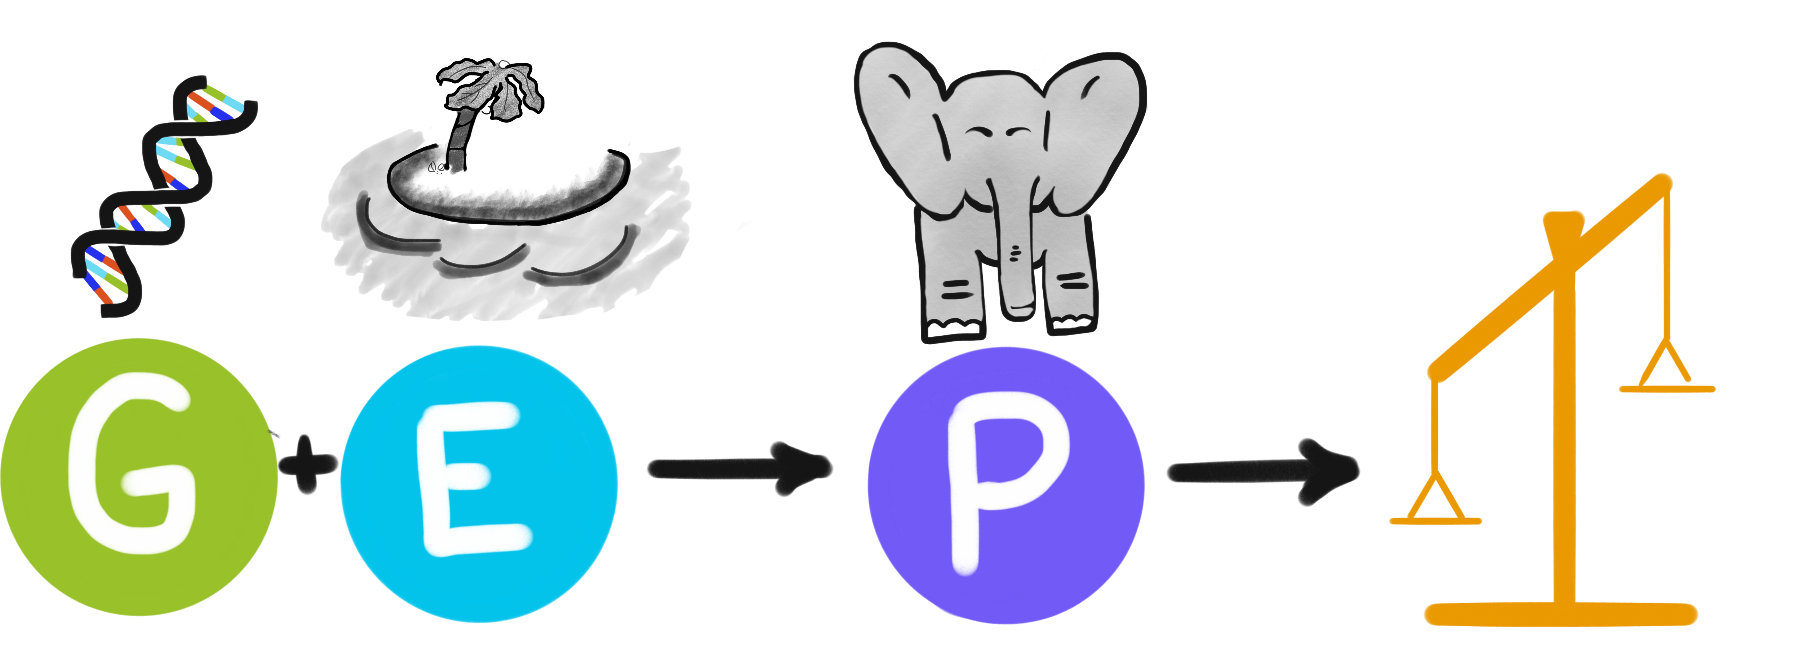
\includegraphics[width=0.6\textwidth]{img/bioscheme}
    \caption{biological inspiration}
    \label{subfig:bioscheme}
  \end{subfigure}
  \hfill
  \begin{subfigure}[b]{0.6\textwidth}
    \centering
    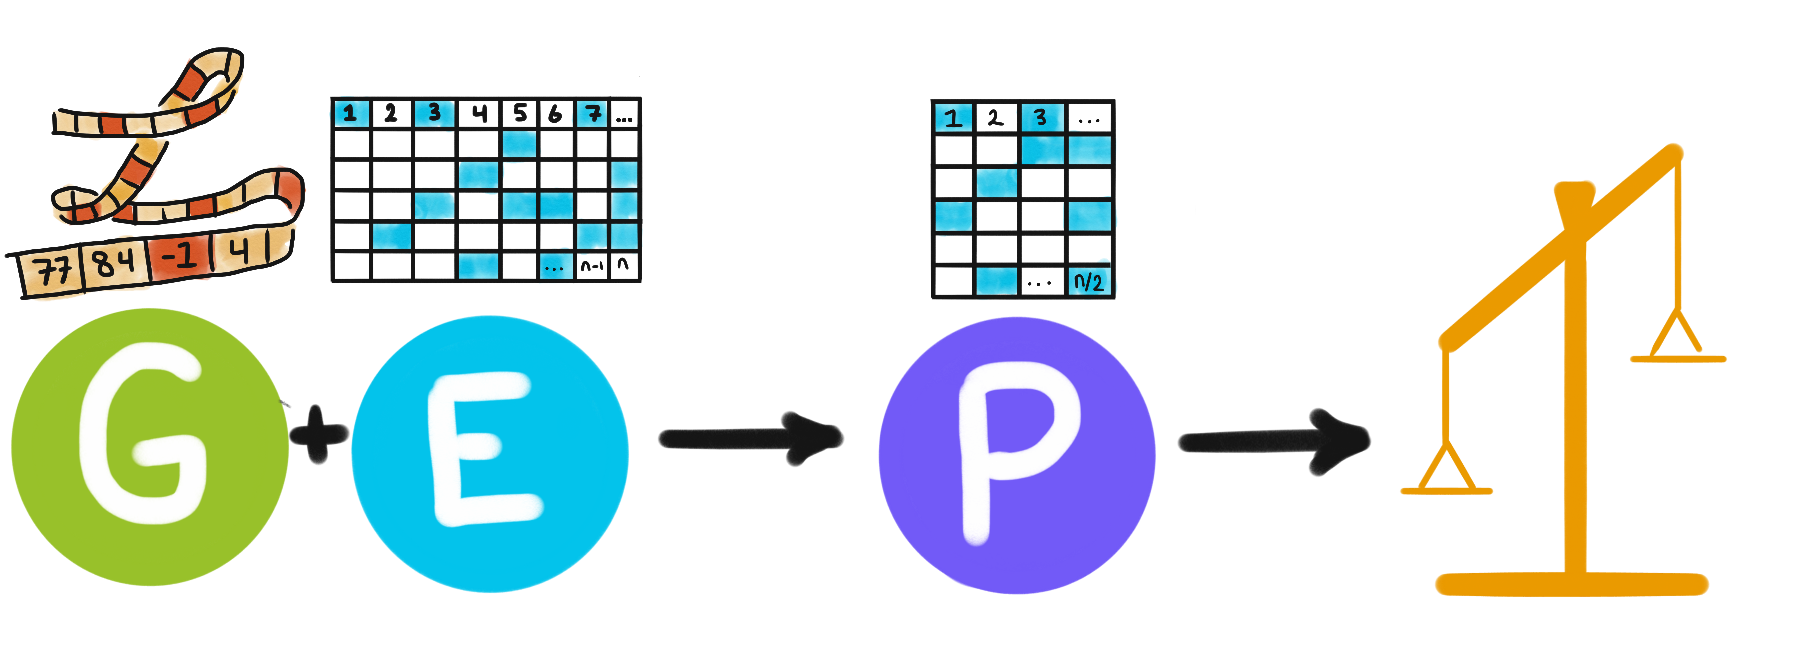
\includegraphics[width=\textwidth]{img/modelscheme}
    \caption{genetic regulatory network model}
     \label{subfig:modelscheme}
  \end{subfigure}
  \captionsetup{singlelinecheck=off,justification=raggedright}
  \caption{A comparison of the genetic regulatory network model and its biological inspiration.}
  \label{fig:model_bio_comparison}
\end{figure}
\end{frame}

\begin{frame}{Model Implementation}
\begin{columns}
\begin{column}{0.6\textwidth}
\begin{itemize}
\item model implemented through DEAP (Distributed Evolutionary Algorithms in Python) framework \cite{Fortin2012DEAP:Easy}
\item experiments performed and analyzed on remote clusters using Jupyter notebook
\end{itemize}
\end{column}
\begin{column}{0.4\textwidth}
\begin{center}
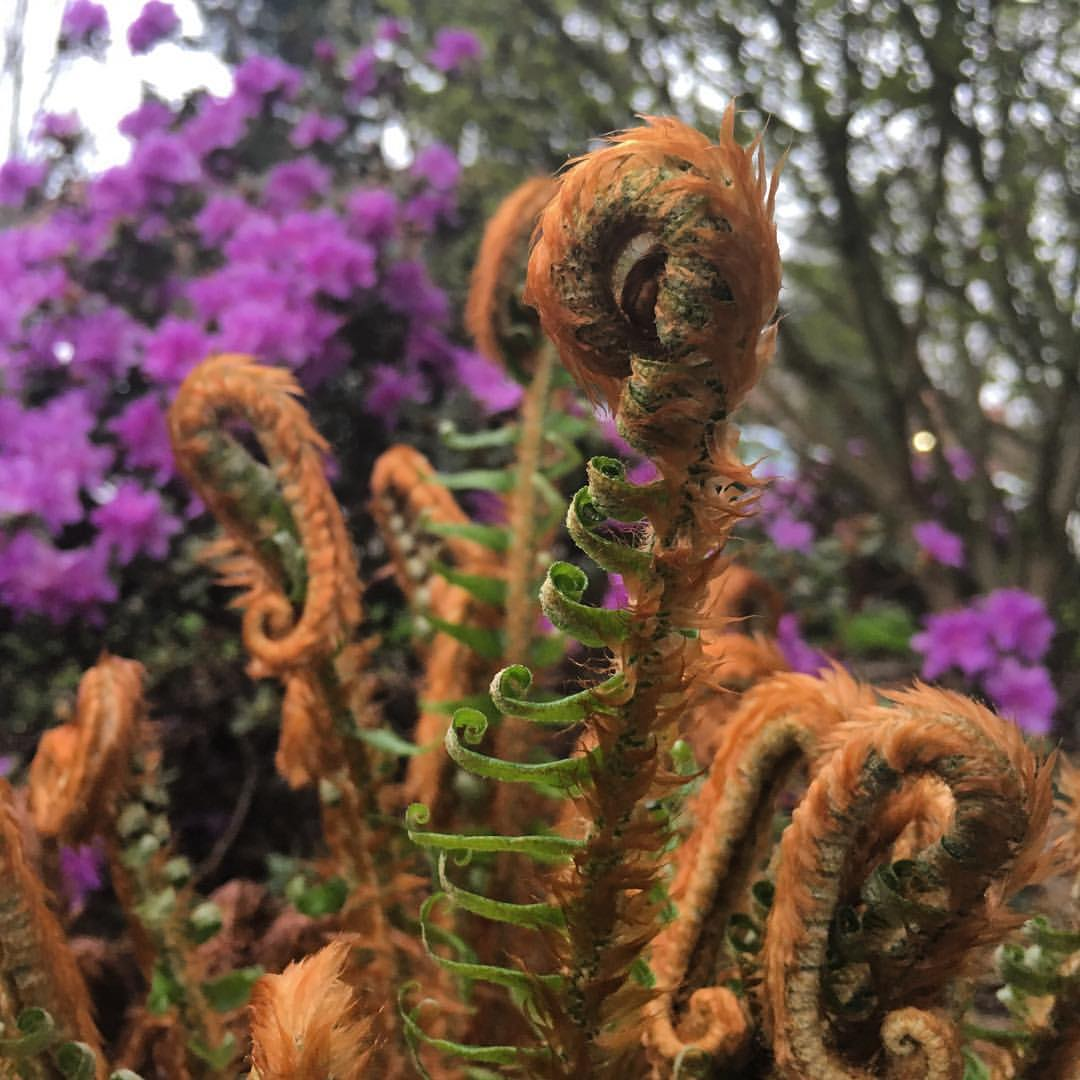
\includegraphics[width=\textwidth,trim={6cm 0 6cm 0},clip]{img/fuzzy_fern}
\end{center}
\end{column}
\end{columns}
\end{frame}




